\chapter{Additional R Diagnostic and E3 Image Archive}
\label{app:e3_archive}

\section{Additional R Executions and Source Precision}
\begin{table}[tbp]\centering\footnotesize
\caption[Additional R diagnostic runs]{All five \(R^{*}\) executions on 19 October, at the report's printed per-run precision. The first diagnostic precedes four extension runs. These do not replace the original R1--R5. Time is first automatic procedure completion; pass speed uses the successful loaded-pass support.}
\label{tab:e1_rstar_all}\begin{tabular}{lrrrr}
\toprule
Run & Time (s) & $J_{\mathrm{excess}}$ (N\,s) & Peak (N) & Pass (mm/s) \\
\midrule
R$^{*}$1 & 22.481 & 0.000 & 21.488 & 10.696 \\
R$^{*}$2 & 25.319 & 0.000 & 22.000 & 10.887 \\
R$^{*}$3 & 25.520 & 0.000 & 20.541 & 10.886 \\
R$^{*}$4 & 25.458 & 0.000 & 22.727 & 10.822 \\
R$^{*}$5 & 25.420 & 0.000 & 20.944 & 10.915 \\
\bottomrule
\end{tabular}

\end{table}

The source is the 17-page additional-R report, pp.1--5 and 17. It records separate configuration identifiers for the first diagnostic and four extension runs, preserved in \path{data/e1_rstar_report_runs.csv}, with the same frozen template, feed, runtime source, +18 N target, and v2 evaluator/observer. The separate configuration/session identifiers document the one-then-four history. The original input manifest, template file/hash, and full per-run CSV/run identifiers could not be reopened in this revision environment; agreement beyond the report's printed precision is not asserted.

Reaggregation of the printed times gives 24.8396 s and sample SD 1.320516 s, agreeing on rounding with the report's authoritative \EoneRstarTime\(\pm\)\EoneRstarTimeSD~s. The current summary retains that published precision rather than implying recovery of the original unrounded values. All five zero excess integrals and the unusually short first run remain included.

\section{E3 Main-Run Pixel Areas}
\begin{table}[tbp]\centering\footnotesize
\caption[Individual E3 main-run image areas]{All 20 main selected N/P1/D1/D2 runs. Areas are exact integer pixel counts printed on pp.5--9 of the 39-page report; percentages are recomputed using Equation~\eqref{eq:e3_removal}. D1-4's final area and percentage remain null. Image evaluability is not procedure success.}
\label{tab:e3_all_runs}\begin{tabular}{lrrrl}
\toprule
Run & $A_{\mathrm{before}}$ (px) & $A_{\mathrm{after}}$ (px) & Removal (\%) & Note \\
\midrule
N-1 & 837 & 0 & 100.000 & image evaluable \\
N-2 & 879 & 0 & 100.000 & image evaluable \\
N-3 & 699 & 0 & 100.000 & image evaluable \\
N-4 & 697 & 0 & 100.000 & image evaluable \\
N-5 & 712 & 0 & 100.000 & image evaluable \\
P1-1 & 858 & 31 & 96.387 & image evaluable \\
P1-2 & 846 & 6 & 99.291 & image evaluable \\
P1-3 & 772 & 11 & 98.575 & image evaluable \\
P1-4 & 846 & 2 & 99.764 & image evaluable \\
P1-5 & 799 & 50 & 93.742 & image evaluable \\
D1-1 & 546 & 41 & 92.491 & image evaluable \\
D1-2 & 676 & 0 & 100.000 & image evaluable \\
D1-3 & 680 & 0 & 100.000 & image evaluable \\
D1-4 & 700 & \NA & \NA & tool occlusion \\
D1-5 & 798 & 0 & 100.000 & image evaluable \\
D2-1 & 768 & 79 & 89.714 & image evaluable \\
D2-2 & 738 & 13 & 98.238 & image evaluable \\
D2-3 & 794 & 128 & 83.879 & image evaluable \\
D2-4 & 743 & 13 & 98.250 & image evaluable \\
D2-5 & 684 & 12 & 98.246 & image evaluable \\
\bottomrule
\end{tabular}

\end{table}

The report's per-run identities and areas are captured in \path{data/e3_report_area_runs.csv}. The exact per-run ratios reproduce the reported main condition means and sample SDs. P1 ranges from 93.742 to 99.764\%, evaluable D1 from 92.491 to 100.000\%, and D2 from 83.879 to 98.250\%. The eight 100\% observations (five N and D1-2/3/5) mean black-ink nondetection under the established criterion.

\section{Occlusion, Interruption, and P2 Exclusion}
\begin{table}[tbp]\centering\footnotesize
\caption[Executed P2 archive records]{P2 was executed five times and remains in the original 25-run selection. Every final photograph is tool-occluded. The initial areas are retained; whole-stain final areas and removal percentages are unavailable, not zero. P2 is outside the main four-condition removal evaluation.}
\label{tab:e3_p2_archive}\begin{tabular}{lrrl}
\toprule
Run & $A_{\mathrm{before}}$ (px) & Image result & Original stop \\
\midrule
P2-1 & 777 & unavailable & \texttt{operator\_finish} \\
P2-2 & 773 & unavailable & \texttt{operator\_finish} \\
P2-3 & 652 & unavailable & \texttt{operator\_finish} \\
P2-4 & 717 & unavailable & \texttt{operator\_finish} \\
P2-5 & 778 & unavailable & \texttt{operator\_finish} \\
\bottomrule
\end{tabular}

\end{table}

D1-4 retains \texttt{manual\_abort}; its interruption-time diagnostic frame contains visible residual marking and final tool occlusion. The report identifies the frame as received 34.5 ms before the abort request (source stamp approximately 0.55 s before it). No post-HOME photograph is available. The visible region is not used to estimate hidden total residual area. P2's initial frames are same-run pre-execution raw RGB, replacing initially occluded photographs; the final occlusion remains. These records are not removed or renamed in the archive.

\begin{figure}[tbp]\centering
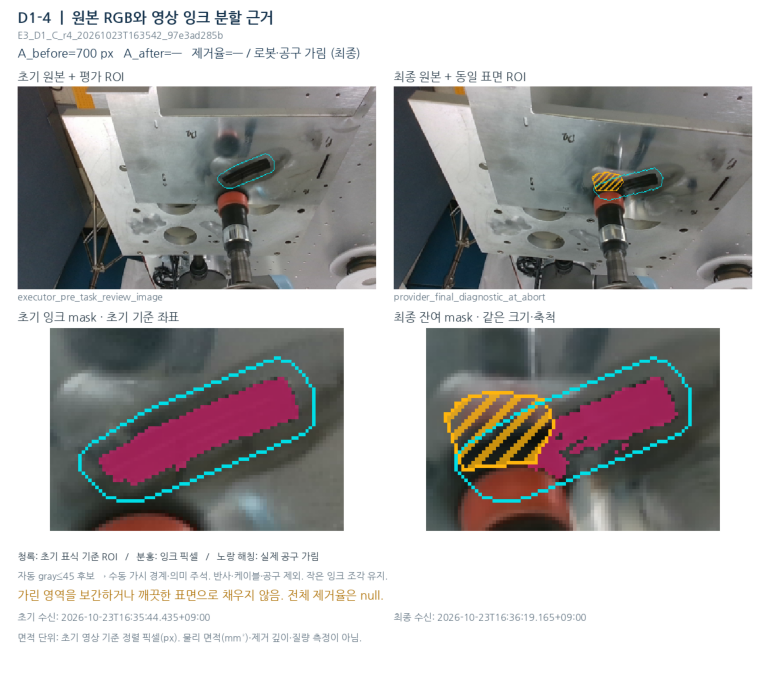
\includegraphics[width=.88\linewidth]{figures/e3_D1-4_report_evidence.png}
\caption[D1-4 retained interruption and occlusion evidence]{Unchanged report-embedded D1-4 evidence, from p.28. Cyan marks the common ROI, magenta denotes annotated visible ink, and hatching indicates tool occlusion. The visible residual and original interruption are preserved; the whole-stain final area is unavailable. This is a report reproduction, not a newly registered or resegmented image pair.}
\label{fig:e3_d1_occlusion}
\end{figure}

\begin{figure}[tbp]\centering
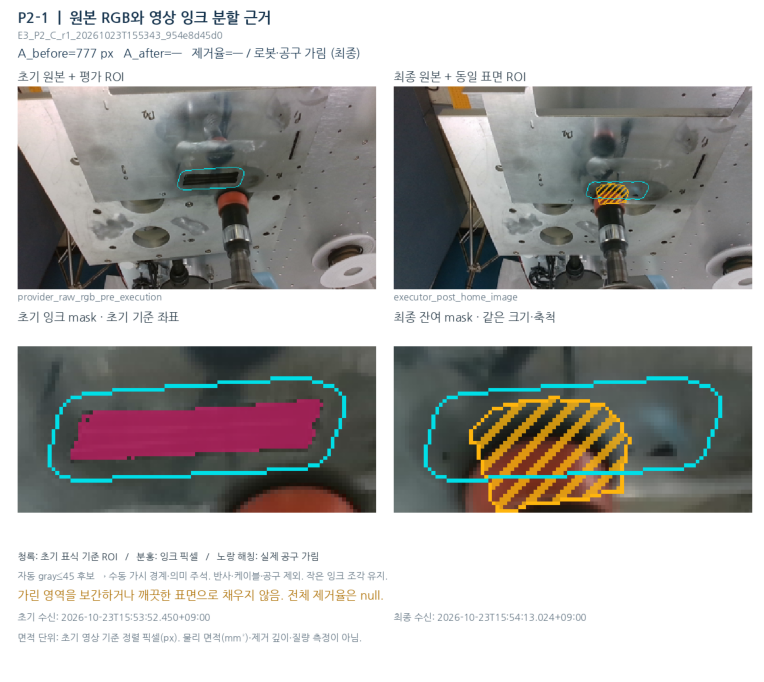
\includegraphics[width=.88\linewidth]{figures/e3_P2-1_report_evidence.png}
\caption[P2 retained final occlusion example]{Unchanged P2-1 report evidence, p.20. Its pre-execution replacement initial image exposes the stain, while final tool occlusion prevents whole-stain removal measurement. All five P2 panels are retained in the supplied evidence archive; P2 is not an unexecuted condition.}
\label{fig:e3_p2_occlusion}
\end{figure}

\section{Reused Segmentation Sensitivity and Procedure Diagnostics}
The report's sensitivity check keeps annotations and ROI fixed and changes the gray threshold equally in before/after images. The published condition means are reproduced below at their printed precision; no new threshold or manual boundary is selected.

\begin{table}[tbp]\centering\small
\caption[Archived E3 threshold sensitivity]{Existing sensitivity results from the image report, p.36. Values are condition-mean percentages; main gray threshold is 45. These are not sample SD or confidence intervals. D1 uses four images throughout.}
\label{tab:e3_sensitivity}
\begin{tabular}{lrrr}\toprule
Condition & gray \(\leq40\) & gray \(\leq45\) & gray \(\leq50\) \\ \midrule
N & 100.000 & 100.000 & 100.000 \\
P1 & 97.912 & 97.552 & 96.914 \\
D1 & 98.124 & 98.123 & 98.056 \\
D2 & 94.659 & 93.665 & 92.932 \\
\bottomrule\end{tabular}
\end{table}

The old v2 procedure outcomes, reproduced on p.37 of the image report, are 8 completed and 17 \texttt{observation\_unavailable} in the original 25-run selection, with 24/25 HOME returns. These are auxiliary diagnostic labels on that archive, not removal successes or outcomes for the main 20-run subset. Image inclusion is independent of them. The original execution report and its full force/path CSV were not present locally; this revision cites the preserved image-report diagnostic summary without claiming a new calculation.

\section{Evidence Availability and Reproduction}
The 39-page report's pp.10--34 contain one before/after RGB, ROI, mask, and occlusion evidence panel per selected run. All 25 embedded panels are losslessly extracted to \path{provenance/results_20261103/e3_report_panels/}. The panel manifest maps each to its original run identifier and report page. The main figure uses repeat 1 of each main condition, with fixed identical crop rectangles documented by the regeneration script. These are display operations on existing report images and are never input to area measurement.

The report describes \path{image_pair_manifest.json} and its CSV counterpart, \path{analysis_config.json}, \path{annotations.json}, \path{occluded_runs.csv}, and the per-run raw RGB/ROI/mask files in the research repository. Those originals were not accessible on this PC. Thus this revision recovers exact printed integer-area statistics and unchanged photographic evidence at report level, while original file-path/hash and annotation reproduction remain document-source checks that cannot be claimed complete. The supplied four original PDF reports are preserved byte for byte. Registered E3 offsets and common-checkpoint/termination details additionally follow the user's confirmed revision record and are identified as such in the source map.
